\section{Introduction}

Data visualisation is essential to data science and science communication. The
power of data visualisation as a communicative tool means it is also open to
misinterpretation and misuse: patterns in raw data can be obscured, statistical
assumptions hidden, and effect sizes misrepresented \cite{weissgerber15}. These
concerns can be addressed in part through improved statistical practices and
novel plot and chart designs \cite{allen19}, but also by making visualisations
themselves more open and explorable \cite{dragicevic19}.

An important aspect of explorability that has been studied for several decades
are techniques for helping the user grasp how a visualisation relates to other
concurrent visualisations of the same underlying data. For example,
geoscientists often work with multiple layered views. To show how these are
related, spatial analytics applications like GeoDa \cite{anselin06} can
automatically select the relevant part of one view as the user changes the
selection in a related view, say a choropleth map. [This is funky because...]

However, this feature is available only if it was specifically anticipated by
the application or library developer; if the geoscientist uses custom libraries
or wants other views linked that the developer did not onsider, they are out of
luck.

\begin{figure}[H]
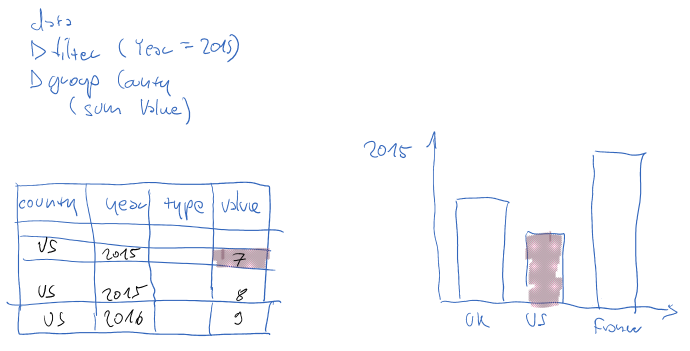
\includegraphics[scale=0.35]{image/chart-fwd}
\caption{Forward linking from code and data to visualisation}
\end{figure}

In this short paper, we present a framework for authoring visualisations where
support for linking is built in, making this powerful comprehension feature
automatic. Moreover, [between data, code, and visualisations.]

\cite{becker87,buja91}
